\documentclass[11pt]{article} 
\usepackage{multicol}
\usepackage{graphicx}
\usepackage{lineno}
\usepackage{lscape}
\usepackage{hyperref} 
\usepackage{apacite}
\usepackage{booktabs}
\usepackage{enumitem}  
\usepackage{tikz}
\usepackage{caption}
\usepackage{subcaption}
\usepackage{float}

\usetikzlibrary{positioning, fit, calc}   
\tikzset{block/.style={draw, thick, text width=2cm ,minimum height=1.3cm, align=center},   
line/.style={-latex}     
} 

\begin{document}
\begin{center}


\includegraphics[scale=0.52]{mmu_logo.png}\\
\vspace{1.0cm}
\Large{\textbf{TDS 3301 \\DATA MINING}} \\
\vspace{1.5cm}
\Large{\textbf{INSURANCE PRODUCT RECOMMENDATION}} \\
\vspace{1cm}
 


\vspace{6.cm}
\normalsize{Prepared by} \\
\vspace{2.5cm}
\large{\textbf{Lou Jia Yu 1161104266 0133502907}} \\ 
\large{\textbf{Perivitta A/P Rajendran 1171101579 0165260944}} \\ 
\large{\textbf{Sarah Batrisyia binti Ahmad Salman 1181301724 01165583004}} \\ 

\end{center}

\thispagestyle{empty}
 
\clearpage 

% ============================================

\section{Introduction}
\textrm{\hspace{1cm}For this project, we have decided to implement the Insurance Product Recommendation. The data set that we will be using is the 'insurance.csv' which consist of 500 rows and 24 columns. Below is the description of the variables that are included in our data set: }


\begin{multicols}{2}
\begin{itemize}
    \item Age
    \item Gender
    \item MaritalStatus
    \item SmokerStatus
    \item LifeStyle
    \item LanguageSpoken
    \item HighestEducation
    \item Race
    \item Nationality
    \item MalaysiaPR
    \item MovingToNewCompany
    \item Occupation
\end{itemize}
 \columnbreak
\begin{itemize}
   
    \item Telco
    \item HomeAddress
    \item ResidentialType
    \item NoOfDependent
    \item FamilyExpenses(month)	
    \item AnnualSalary
    \item Customer\_Needs\_1
    \item Customer\_Needs\_2
    \item PurchasedPlan1
    \item Transport
    \item PurchasedPlan2
    \item MedicalComplication

\end{itemize}
\end{multicols}
\textrm{\hspace{1cm}Most of the variables that was provided in the data set is understandable and clearly described. For this project, we focused more on the Customer\_Needs\_1 (the primary need of the customer), Customer\_Needs\_2, (The secondary requirement of a customer), PurchasedPlan1 (Available plans under the Customer\_Needs\_1), and PurchasedPlan2 (Available plans under the Customer\_Needs\_2). Below, we will further explain step-by-step on how our project was carried.}


\vspace{1.0\baselineskip} 

\section{Exploratory Data Analysis}

\begin{center}

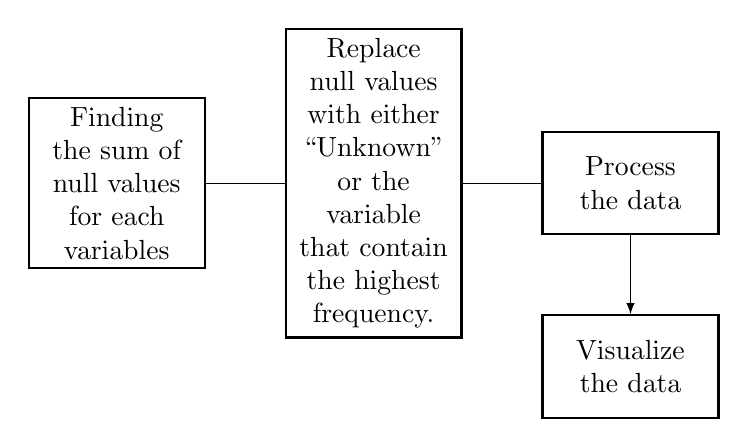
\begin{tikzpicture}[node distance=1cm]
\node[block] (Process 1) {Finding the sum of null values for each variables};  
\node[block,right=of Process 1] (Process 2) {Replace null values with either ``Unknown" or the variable that contain the highest frequency.};   
\node[block,right=of Process 2] (Process 3) {Process the data};  
\node[block,below=of Process 3] (Process 4) {Visualize the data}; 

\draw[line] (Process 1)-- (Process 2)-- (Process 3)-- (Process 4);  
\end{tikzpicture}
\end{center}

Overall work for Exploratory Data Analysis (EDA) is shown in the figure above. The work began with finding, sum of null values for each variable. Null values can mostly impact the outcomes of a data set. In order for us to handle the null values, we started off by replacing the null values with either ``Unknown" or the variable that contains the highest frequency or the mean or median of the variable. ``Unknown" is known as the global constant in handling missing data. Next is followed by processing the data. Label encoding has been performed in the data set for us to further analyze in the future. The original data set has been copied for us to perform data mining techniques without changing the data set. Lastly we continued to do visualization for our data set before applying any data mining techniques to see if there is any relationship or pattern that can be further analyze using data mining techniques.

\subsection{Missing Value Treatment}

\hspace{0.5cm}The method that we have used to solve the missing values are by assuming the NaN value for Occupation is ``Unemployed" and the SmokerSatus as ``Non-Smoker". \vspace{0.3cm}

\hspace{0.5cm}{Additionally, we replaced the null(NaN) value by applying value\_counts function to get the highest frequency of the variable and we replaced to NaN value. For instance, we replaced the NaN value of the variable ``HomeAddress" to ``central\_mal". }\vspace{0.3cm}

\hspace{0.5cm}{Besides that, if the unique value frequency of the variable does not make a huge differences, then we replace the NaN values to ``Unknown". As for the attributes like ``Nationality', ``MaritalStatus', and ``Race' we have replaced the NaN value to "Unknown".} 

 
\subsection{Feature Engineering}

\hspace{0.5cm}The extra features that we have added in this project is the label encoding method. Label encoding lies under the ordinal encoding where the order of data matters. Each category will be assigned to a value from 1 to N, where N is the number of category in the attribute. The label encoder will be labelled based on the alphabetical order. If there is any ``Unknown' value in the attributes then it will automatically assign it to the value '0'.\vspace{0.3cm}

\hspace{0.5cm}Next, We continued with label encoding for other attributes such as `MalaysianPR', `MovingToNewCompany', `LifeStyle', `MaritalStatus', `LanguageSpoken', `HighestEducation', `Race', `Nationality', `Telco', `HomeAddress' and `Transport' . For example, the attribute `Gender' after label encoding, it will assign female to 0 while male will be assigned to 1. As for attributes that has either `yes' or `no' will be assigned with values, such as `1' and `0'.The attributes `MalaysianPR' and `MovingToNewCompany' has the values `yes' and `no'.Figure \ref{fig:test} shows the outputs of the attributes after label encoding.

\begin{figure}[H]
\centering
\begin{subfigure}{.5\textwidth}
  \centering
  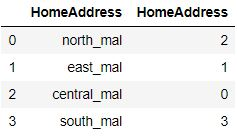
\includegraphics[width=.8\linewidth]{LabelEncodingAddress}
  \caption{HomeAdress}
  \label{fig:LabelEncodingAddress}
\end{subfigure}%
\begin{subfigure}{.6\textwidth}
  \centering
  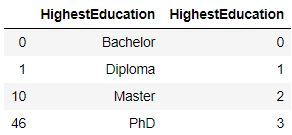
\includegraphics[width=.8\linewidth]{LabelEncodingEdu}
  \caption{HighestEducation}
  \label{fig:LabelEncodingEdu}
\end{subfigure}
%\caption{A figure with two subfigures}
\label{fig:test}
\\
\centering
\begin{subfigure}{.5\textwidth}
  \centering
  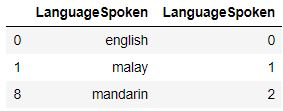
\includegraphics[width=.9\linewidth]{LabelEncodingLanguage}
  \caption{LanguageSpoken}
  \label{fig:LabelEncodingAddress}
\end{subfigure}%
\begin{subfigure}{.5\textwidth}
  \centering
  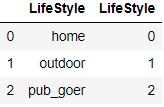
\includegraphics[width=.6\linewidth]{LabelEncodingLifeStyle}
  \caption{LifeStyle}
  \label{fig:LabelEncodingEdu}
\end{subfigure}
%\caption{A figure with two subfigures}
\label{fig:test}

\centering
\begin{subfigure}{.5\textwidth}
  \centering
  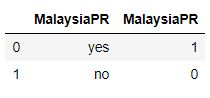
\includegraphics[width=.7\linewidth]{LabelEncodingMalaysianPR} 
  \caption{MalaysianPR}
  \label{fig:LabelEncodingAddress}
\end{subfigure}%
\begin{subfigure}{.5\textwidth}
  \centering
  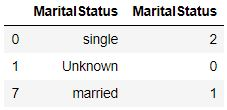
\includegraphics[width=.8\linewidth]{LabelEncodingMaritalStatus}
  \caption{MaritalStatus}
  \label{fig:LabelEncodingEdu}
\end{subfigure}
%\caption{A figure with two subfigures}
\label{fig:test}

\centering
\begin{subfigure}{.5\textwidth}
  \centering
  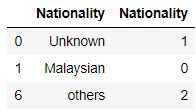
\includegraphics[width=.7\linewidth]{LabelEncodingNationality}
  \caption{Nationality}
  \label{fig:LabelEncodingAddress}
\end{subfigure}%
\begin{subfigure}{.5\textwidth}
  \centering
  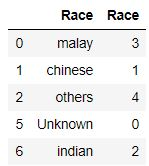
\includegraphics[width=.5\linewidth]{LabelEncodingRace}
  \caption{Race}
  \label{fig:LabelEncodingEdu}
\end{subfigure}
%\caption{A figure with two subfigures}
\label{fig:test}

\centering
\begin{subfigure}{.5\textwidth}
  \centering
  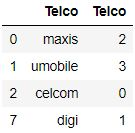
\includegraphics[width=.5\linewidth]{LabelEncodingTelco}
  \caption{Telco}
  \label{fig:LabelEncodingAddress}
\end{subfigure}%
\begin{subfigure}{.5\textwidth}
  \centering
  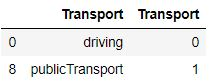
\includegraphics[width=.8\linewidth]{LabelEncodingTransport}
  \caption{Transport}
  \label{fig:LabelEncodingEdu}
\end{subfigure}
\caption{After Label Encoding}
\label{fig:test}

\end{figure}

\section{Feature Selection}
\hspace{0.5cm}From the data set, we performed two feature selection which is BORUTA and Recursive Feature Elimination (RFE). We have included attributes of `Age', `Gender', `NoOfDependent', `FamilyExpenses(Month)', `AnnualSalary', `MedicalComplication', `MaritalStatus' for Unknown, married, and single, `SmokerStatus' for nonsmoker, frequent and once in a while.\vspace{0.3cm}

\hspace{0.5cm}The first feature selection that we used is BORUTA. From the given data set, it will be randomised and resulted a shuffled copies of the features. The extended data set will then be trained with a random forest classifier and a feature importance measure. It will be applied to evaluate the importance of each feature where it considers more important features if the score is high. This process will repeat to check if a real feature has higher importance than the best and will removes those which are deemed highly unimportant. The algorithm will stop once all of the features get confirmed or rejected or if it has reaches a specified limit of random forest runs. We chose BORUTA as one of the feature selection because it will lead to a minimal optimal subset of features as the method minimizes the error of random forest model. BORUTA is also known for it ability to handle interactions between variables. By using BORUTA we are able to see the top features that has the highest.\vspace{0.3cm} 

\hspace{0.5cm} The next feature selection that we used is the Recursive Feature Elimination (RFE). RFE will fit a model and removes the weakest features until the specified number of features is reached. RFE is known to be used on large feature sets and it does not require any knowledge of the representation of the features. We used RFE on the same dataset that we used on BORUTA because we wanted to see the differences of the both outcomes and see which feature selection shows the best results.\vspace{0.3cm}

\hspace{0.5cm} Based on the two feature selection method that we've used, RFE seems to be the optimal method. We will further discuss this in the findings below. 


\subsection{Feature Modeling}
\hspace{0.5cm} We handled the imbalanced data by implementing SMOTE to balance the data. The first step we performed, is that we applied label encoding which only contains '0' and '1' indicating as either ``No" and ``Yes", respectively on the variable ``Medical Complication". \vspace{0.3cm} 

Moreover, we extracted some of the selected attributes such as ``SmokerStatus',``Occupation',``Customer\_Needs\_1", ``Customer\_Needs\_2', ``PurchasedPlan1', ``PurchasedPlan2' that had already applied label encoding in the previous steps. \vspace{0.3cm} 

After extracting all of the needed variables, creating dummy variables were then implemented. ``Medical Complication" was also included as one of the attribute to perform dummy variable technique.\vspace{0.3cm} 

 \begin{figure}[H]
     \centering
     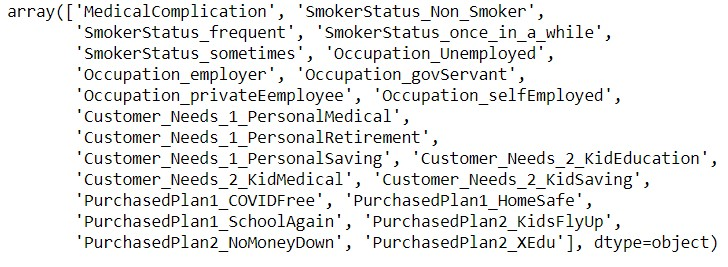
\includegraphics[width=0.85\textwidth]{dummy.jpg}
     \caption{Output of dummy variables}
     \label{fig:dummy.jpg}
 \end{figure}

``Medical Complication" is the target variable for SMOTE. Therefore, for the training set and test set of \emph X included all of the dummy variables except for ``Medical Complication", however, on the other hand, \emph y only included ``Medical Complication". SMOTE is then performed after splitting the training set into 70\% and 30\% of test set. \vspace{0.3cm} 

After splitting the data, the results shows out that the length of the oversampled data is 420 and 210 are both of the number of no medical complication and having medical complication in oversampled data. The proportion of no medical complication and having medical complication is the same which is 0.5. 


 \begin{figure}[H] 
     \centering
     \includegraphics[width=0.85\textwidth]{sample_data.jpg}
     \caption{Result of splitting}
     \label{fig:sample_data.jpg}
 \end{figure}

The optimization terminated successfully and got the function value of 0.646206. Figure \ref{fig:logit.jpg} below shows the result of Logit.

 \begin{figure}[H] 
     \centering
     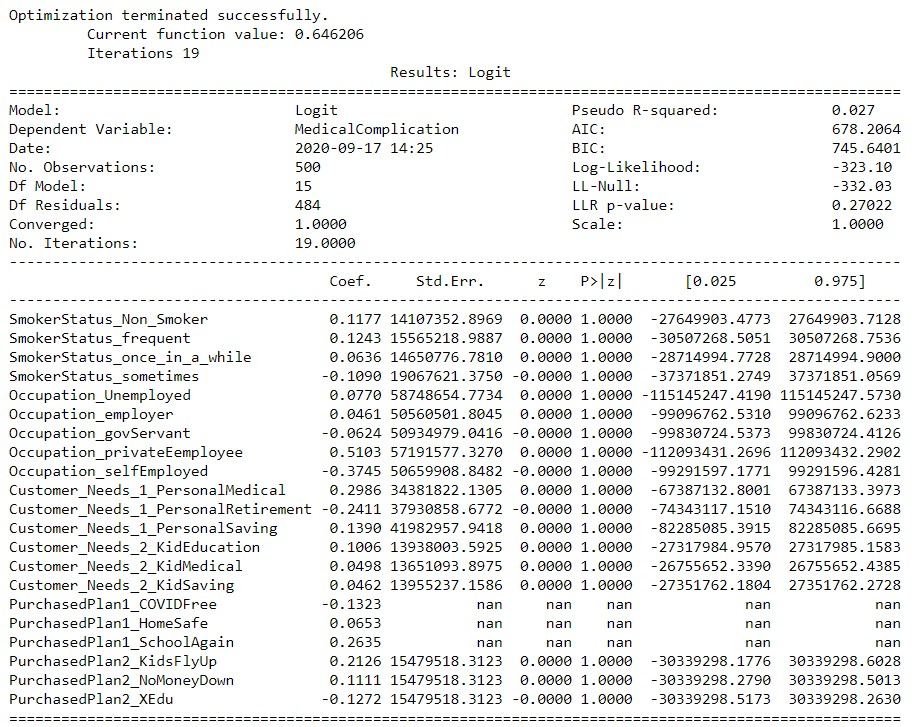
\includegraphics[width=0.85\textwidth]{logit.jpg}
     \caption{Logit Result}
     \label{fig:logit.jpg}
 \end{figure}

\section{Data Mining Techniques}

\hspace{0.5cm} {As for the data mining techniques, we have implemented association rule mining (ARM) and for classification models we have used three different machine learning algorithms such as Logistic Regression (LR), Naive Bayes (NB) and k-Nearest Neighbor (kNN) algorithms. Besides that, we have also applied cluster analysis for the insurance data.}\vspace{0.3cm}


\subsection{Association Rule Mining}
\hspace{0.5cm} {Association rule mining is used to create association rules by searching data for frequent if-then patterns by using two different criteria, where support and confidence is used to identify the most common and important relationships. Confidence indicates the number of times the if-then statements are found true. Next,a method called lift, is used to compare confidence with expected confidence, or how frequently an if-then statement is expected to be found true.}\vspace{0.3cm}

\vspace{0.3cm}{
\hspace{0.5cm}According to our insurance data set, we have constructed association rule mining among selected attributes. The attributes that we have selected for ARM are 'SmokerStatus','LifeStyle', 'Occupation', 'MedicalComplication', 'Customer\_Needs\_1'. The measure of effectiveness on our association rules is to show the correlation among the attributes in the data set because it appears very often but it may occur far less when ARM is applied, depending on the support, confidence and lift values. Using this measures, it helps to separate causation form correlation and allows them to properly value the given value.}

\vspace{0.3cm}{
\hspace{0.5cm}Understanding if the lift value is a negative value, then there is a negative correlation between data points. If the value is positive, there is a positive correlation, and if the ratio equals 1, then there is no correlation. Association rules is useful in our project because it helps on analyzing and predicting customer behaviour and they play an important part in customer analytics.}

\subsection{Classification Models}

\vspace{0.3cm}{
\hspace{0.5cm}NB is a probabilistic machine learning algorithm that can be used in a wide variety of classification tasks. That is because there is a significant advantage with NB. Since it is a probabilistic model, the algorithm can be coded up easily and the predictions made real quick.We have developed Naive Bayes (NB) classification model to predict accuracy of the selected attributes, with the following set of data,'Occupation','FamilyExpenses(month)', and 'AnnualSalary'.}

\vspace{0.3cm}{
\hspace{0.5cm}Initially, we have tested the accuracy of the data set before and after adding the missing values and the accuracy was 31\%. After pre-processing, there is changes with the accuracy, where we have divided, the attributes among categories of `Occupation\_Unemployed', `Occupation\_employer', `Occupation\_govServant', `Occupation\_privateEemployee', `FamilyExpenses(month)', and `AnnualSalary'. The accuracy for occupation as an employer is highest among the rest where it has the value of 93\%, secondly, goverment servant (84\%), thirdly, unemployed (71\%) and private employee with accuracy of (69\%).}

\vspace{0.3cm}{
\hspace{0.5cm}Secondly, LR is a powerful machine learning algorithm that utilizes a sigmoid function and works best on binary classification problems, although it can be used on multi-class classification problems through the `one vs. all' method. We have implemented a logistic regression model to check for the accuracy and we used occupation as our target variable to train the model. Then, we prepped the data, to feed it into the logistic regression classifier, after creating the train and test model. Later on, an instance of the classifier is created and training data has been fitted into to classifier to check for the accuracy. As for the accuracy, it was similar with the output from NB. }

\vspace{0.3cm}{
\hspace{0.5cm} Thirdly, KNN can be used for both classification and regression predictive problems. To evaluate this technique we generally look at 3 important aspects, calculation time, predictive power and ease to interpret output. KNN algorithm fairs across all parameters of considerations. It is commonly used for its easy of interpretation and low calculation time. In order to train the classifier, we set the nearest neighbour value to 5 and then we made the tested the classifier for accuracy. As for the result, KNN's output were slightly different from the other two algorithms where the accuracy for each categorical of occupation, were slightly higher for private employee (71\%) and employee (93\%) with same output. The remaining two outputs had lower accuracy than NB and LG were the unemployed with (63\%) and goverment employee with accuracy of (75\%).}

 \begin{figure}[H]
     \centering
     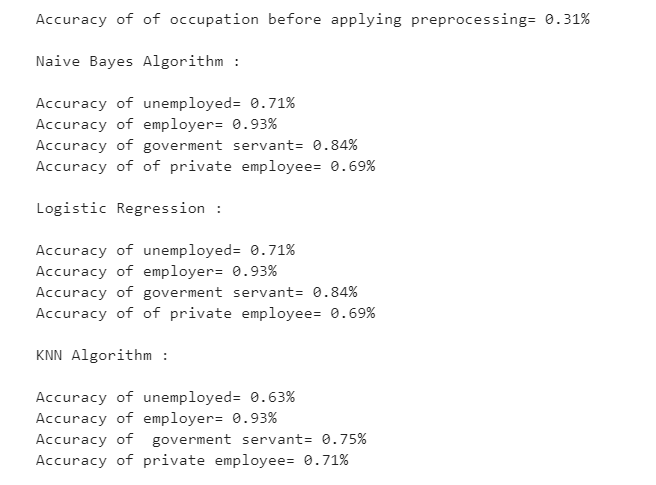
\includegraphics[width=0.85\textwidth]{accuracy.png}
     \caption{Result of Accuracy among LG,KNN and NB}
     \label{fig:accuracy.jpg}  
 \end{figure}


\subsection{Cluster Analysis}
\hspace{0.5cm}The last data mining technique that we have applied in our project is the elbow method. Elbow method is used to determine the number of clusters in a data set. The score of this method is calculated as the mean squared distance between each instance and the closest centroid to it. The elbow method is known as the most intuitive to understand and the easiest to implement. We applied this method on the attributes of ``MovingToNewCompany" and ``MalaysiaPR" that were label encoded. The result of the cluster analysis using the elbow method will be further discuss in the Findings section. 

%----------------------- NEXT SECTION -----------------------
\section{Findings}

\subsection{Exploratory Data Analysis}
\hspace{0.5cm} The intention of people buying insurance is to ensure their safety and body health. Nevertheless, people would not always make their life healthier as there was too many temptation of there such as nicotine. Figure \ref{fig:smoker.jpg} finding below shows that most of the buyers in the data set are smokers. \vspace{0.3cm}

 \begin{figure}[H]
     \centering
     \includegraphics[width=0.85\textwidth]{smoker.jpg}
     \caption{Frequency of Smoker Status}
     \label{fig:smoker.jpg}
 \end{figure}
 
\hspace{0.5cm} On the other hand, we constructed a bar graph to have a review on the smoker status and the first plan that customers want. From the Figure \ref{fig:cn.jpg} below, we could see that most of the smokers aiming to purchase ``Personal Medical", which means that this is good for insurance broker and agent as customers have known that instead of ``Personal Retirement" and ``Personal Saving", they needed ``Personal Medical" the most as nicotine could higher up the risk of sickness. \vspace{0.3cm}

 \begin{figure}[H]
     \centering
     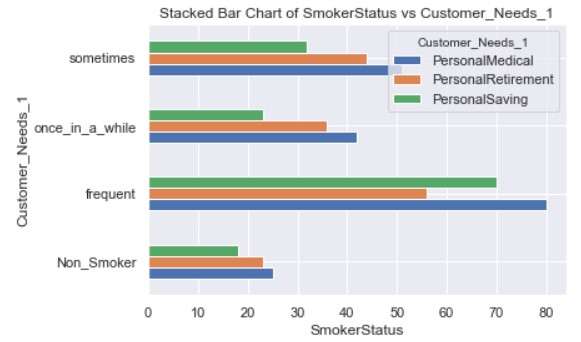
\includegraphics[width=0.85\textwidth]{cn.jpg}
     \caption{SmokerStatus vs Customer\_Needs\_1}
     \label{fig:cn.jpg}
 \end{figure}
\vspace{0.3cm}

\hspace{0.5cm} It is always important to know the policy of customers having on hand currently. Therefore, we construct a graph to study the policy they are having in order to suggest them a better plan. From the Figure \ref{fig:pp.jpg} below, we could see that ``Older\_Adult" really lacked of investment plan which is the ``NoMoneyDown" plan. It is always a benefit to ``Older\_Adult" to purchase ``NoMoneyDown" plan as this could be their new interest after they have retired. It is also an advantages for ``Teenager" and ``Mid\_Aged\_Adult" to invest their funds into investment plan because it could gives them and their family members as a side income. \vspace{0.3cm}

 \begin{figure}[H] 
     \centering
     \includegraphics[width=0.85\textwidth]{pp.jpg}
     \caption{PurchasedPlan2 vs Age\_Bins}
     \label{fig:pp.jpg}
 \end{figure}
\vspace{0.3cm}


\hspace{0.5cm}  Moreover, we explored variable ``Occupation" and ``Customer\_Needs\_1" to have a discover on the needed plan of the customers depends on their occupation. As the Figure \ref{fig:occ.jpg} shown as below, unemployed customers should focus on ``Personal Saving" as they could still have a saving income whenever they are unemployed. Most importantly from the figure below, recommended that self-employed customers should purchase ``Personal Retirement" because they do not have Employees Provident Fund (EPF) as their retirement fund. 

 \begin{figure}[H] 
     \centering
     \includegraphics[width=0.85\textwidth]{occ.jpg}
     \caption{Occupation vs Customer\_Needs\_1}
     \label{fig:occ.jpg}
 \end{figure}
\vspace{0.3cm}

\subsection{Feature Selection}
\hspace{0.5cm} As stated in the feature selection part above, we have performed a feature selection using BORUTA and Recursive Feature Elimintation (RFE). We stated that RFE is the optimal method because based on the Figure \ref{fig:boruta.jpg} and Figure \ref{fig:rfe.jpg}, RFE is effective in selecting features from the trained dataset that are most relevant in predicting the target variable.

 \begin{figure}[H] 
     \centering
     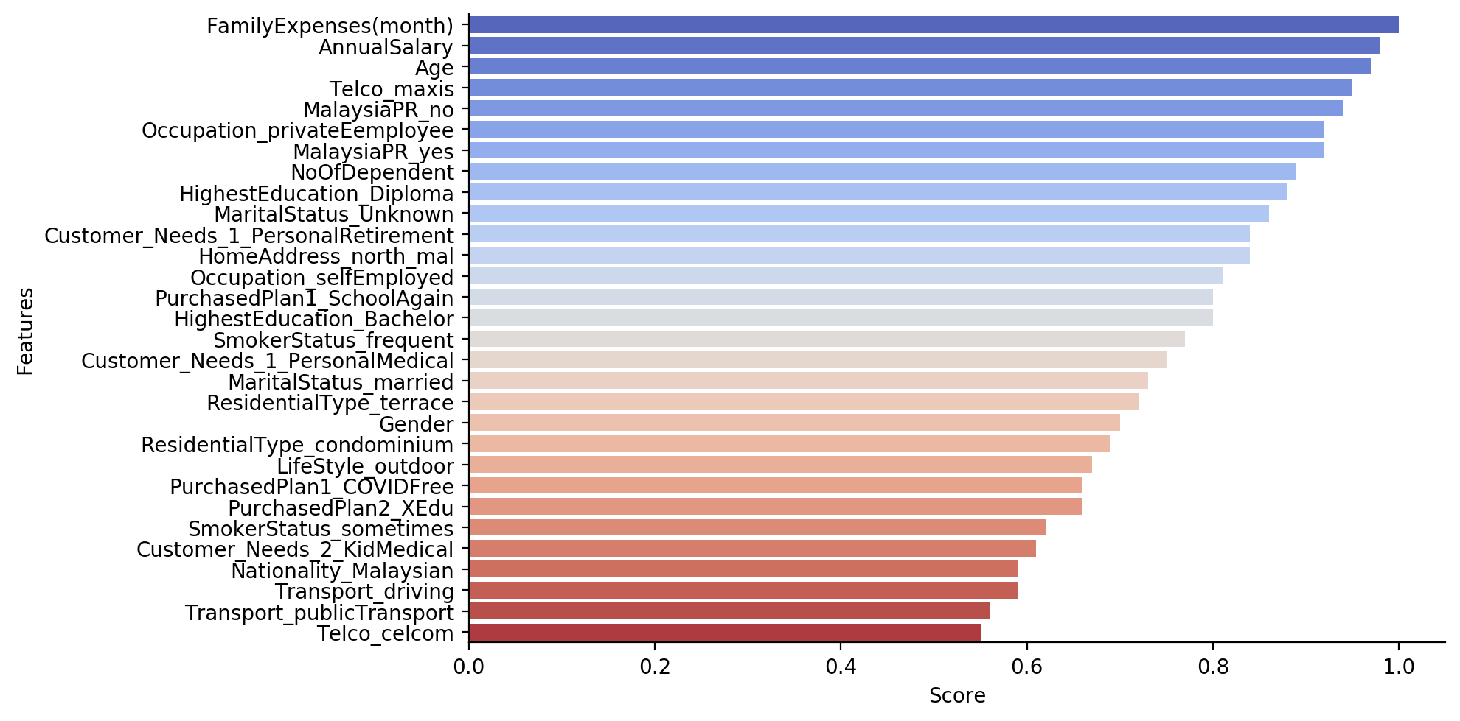
\includegraphics[width=1.2\textwidth]{boruta.jpg}
     \caption{BORUTA Top 30 Features}
     \label{fig:boruta.jpg}
 \end{figure}

\begin{figure}[H] 
     \centering
     \includegraphics[width=1.2\textwidth]{rfe.jpg}
     \caption{RFE Top 30 Features}
     \label{fig:rfe.jpg}
 \end{figure}

\hspace{0.5cm} From the Figures above, it shows a different outcome for both feature selection method. For BORUTA, `FamilyExpenses(month)' seems to be at first while in RFE, `Age' is located in first place. Feature selection is done to tell us features that contribute the most to the prediction variable. As we think about it, `Age' might be one of the features that can contribute the most to the prediction. 

\subsection{Cluster Analysis}

\hspace{0.5cm} 
Cluster Analysis is performed to find similarity between a pair of subjects. From Figure \ref{fig:elbowm.jpg} below, we have perform elbow method on label encoded features of `MovingToNewCompany' and `MalaysiaPR'. From the figure, we can conclude that the optimal number of cluster for the features `MovingToNewCompany' and `MalaysiaPR' is 3.

\begin{figure}[H] 
     \centering
     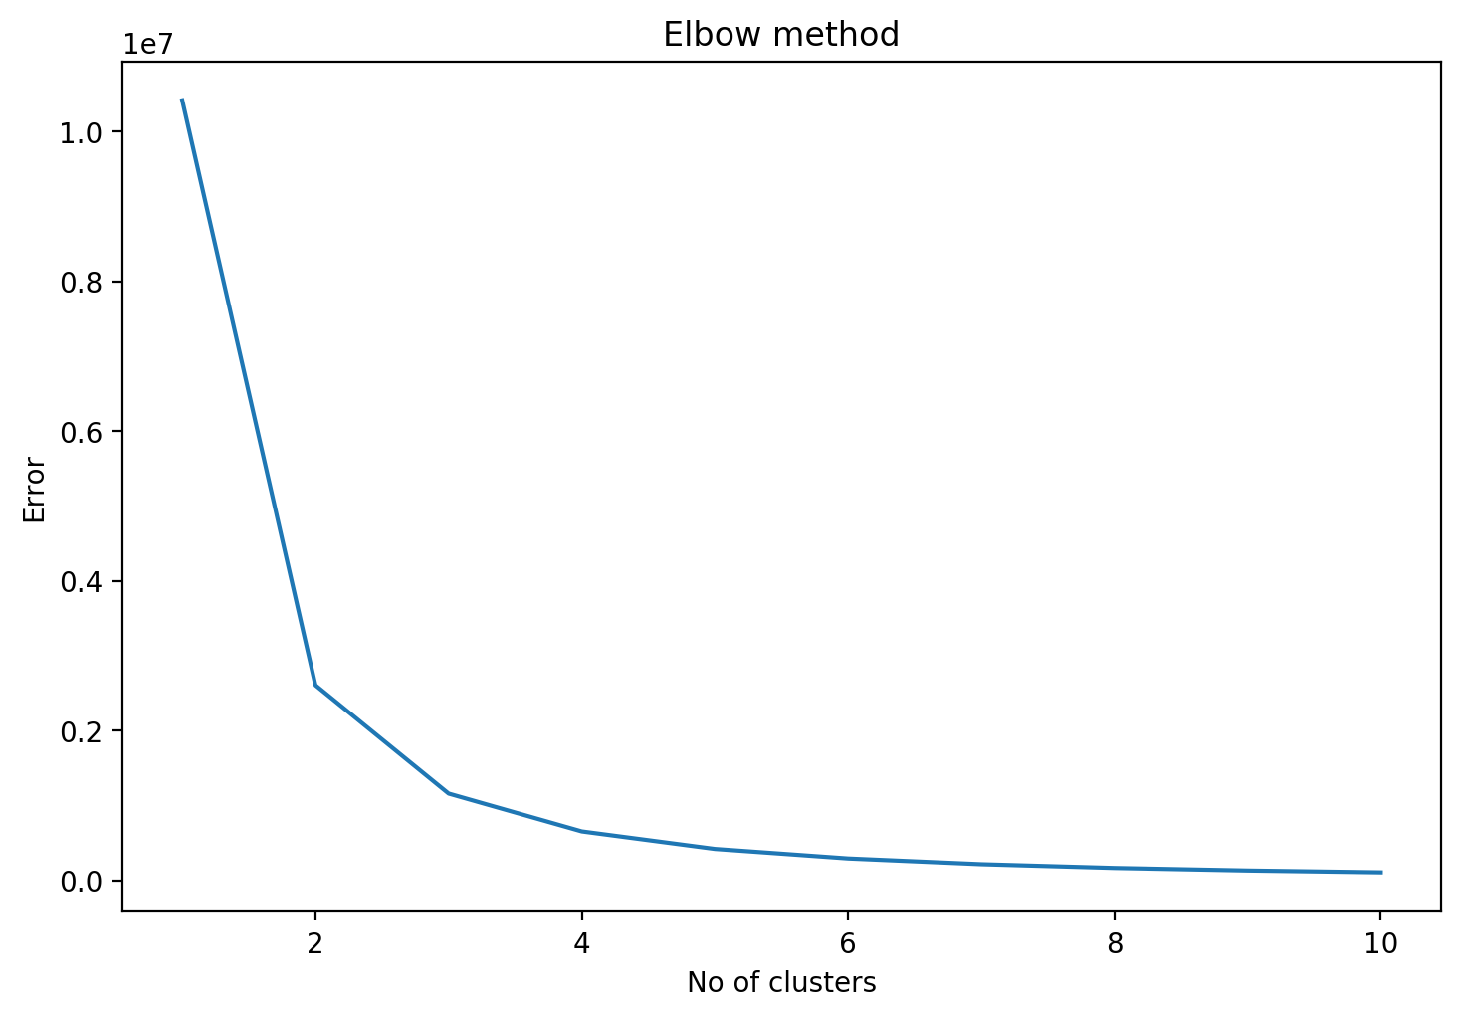
\includegraphics[width=1.0\textwidth]{elbowm.jpg}
     \caption{Elbow Method}
     \label{fig:elbowm.jpg}
 \end{figure}
\vspace{0.3cm}

\subsection{Accuracy Measurement}

\hspace{0.5cm}
According to our project, we have discovered the results of all three algorithms, starting from the analysis of the training and testing data set of the output values. Figure \ref{fig:Table.jpg} below shows the differences of results within three algorithms NB, LG and KNN.

\begin{figure}[H]
     \centering
     \includegraphics[width=1.1\linewidth]{table1.png}
     \caption{Result of Accuracy among LG,KNN and NB}
     \label{fig:Table.jpg}  
\end{figure}
 

\hspace{0.5cm}  We can see that, occupation as an employer has the highest accuracy among all the sub-categories of occupation, and the second highest is government servant. Not only that, the accuracy of LG and NB algorithm has the constant accuracy for the selected attributes compared to KNN algorithm, there is slight difference in terms of accuracy. The changes in accuracy might be due to speed or performance of the respective algorithm. After getting the results from accuracy model, we have selected the top most two occupation (Employer and Government Servant) for further analysis. We continued observing with classification report to measure the quality of predictions from a classification algorithm. How many predictions are True and how many are False. More specifically, True Positives (TP), False Positives (FP), True negatives (TN) and False Negatives(FN).The report shows the main classification metrics precision, recall and f1-score on a per class basis. The metrics are calculated by using true and false positives, true and false negatives. Positive and negative in this case are generic names for the predicted classes.


\begin{table}[H]
\centering
\caption{Classification report for Employer(\%)}
\label{Classification report for Employer(\%)}
\begin{tabular}{p{3cm}p{2cm}p{2cm}p{2cm}p{2cm}}
\hline
            & \multicolumn{3}{c}{Classification (\%)}           \\ \hline
             & precision & Recall    & F1-score & Support       \\ \hline
0            & 0.93      & 1.00      & 0.96    & 139            \\ 
1            & 80        & 82        & 90      & 80             \\ \hline 
accuracy                             & 0.93    & 150            \\ \hline 
macro avg    & 0.46      & 0.50      & 0.48    & 150            \\ \hline 
weighted avg & 0.86      & 0.93      & 0.89    & 150            \\ \hline 
\end{tabular}
\end{table}


\begin{table}
\centering
\caption{Classification report for Government Servant(\%)}
\label{Classification report for Government Servant(\%)}
\begin{tabular}{p{3cm}p{2cm}p{2cm}p{2cm}p{2cm}}
\hline
            & \multicolumn{3}{c}{Classification report(\%)}     \\ \hline
             & precision & Recall    & F1-score & Support       \\ \hline
0            & 0.84      & 1.00      & 0.91    & 126            \\ 
1            & 0.00      & 0.00      & 0.00    & 24             \\ \hline 
accuracy                             & 0.84    & 150            \\ \hline 
macro avg    & 0.42      & 0.50      & 0.46    & 150            \\ \hline 
weighted avg & 0.71      & 0.84      & 0.77    & 150            \\ \hline 
\end{tabular}
\end{table}


\hspace{0.5cm} 
From the results, the F1-score is a weighted harmonic mean of precision and recall such that the best score is 1.0 and the worst is 0.0. From the score, Occupation as Employer with the class '0' has a closer range to 1.0 compared to Government Servant with class of '0' for F1-Score which means the higher the F1-Score the better it is.
\subsection{Conclusion}

\hspace{0.5cm} 
Putting everything into consideration, the insurance company can recommend more employers and government servants to subscribe for the insurance packages since both the occupation holds the most amount of subscriptions from the data set we have explored so far. Secondly, insurance company could come up with more compromising packages for unemployed and private employees, to get more customers. Besides that, it is always a added benefit to the insurance company on analysing their data as they could get an insight of their customers.In addition, it can also benefit the customers since they can be aware on what type of packages that they lack. At last,the best accuracy model from the overall observation, is NB and LG because both is slightly ahead and they had the same accuracy calculations, unlike KNN. So the performance of both model is acceptable.



\section{Deployment}

In this project, the work is visualized via streamlit. The prototype can be accessed at :\\

    \\  Local URL: http://localhost:8501\vspace{0.3cm}

    \\  Network URL: http://192.168.0.108:8501 \\

Sample screenshots from streamlit are shown below:

 \begin{figure}[H] 
     \centering
     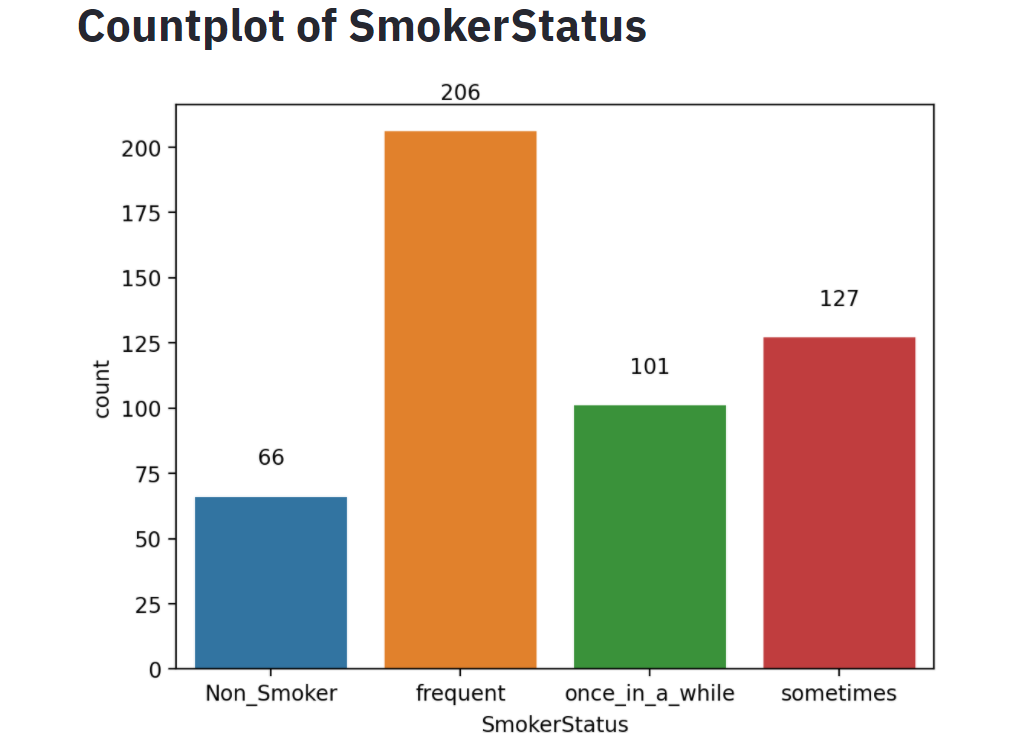
\includegraphics[width=0.95\textwidth]{diagram1.png}
     \caption{Frequency of Smoker Status}
     \label{fig:diagram1.png}
 \end{figure}
\vspace{0.3cm}

 \begin{figure}[H] 
     \centering
     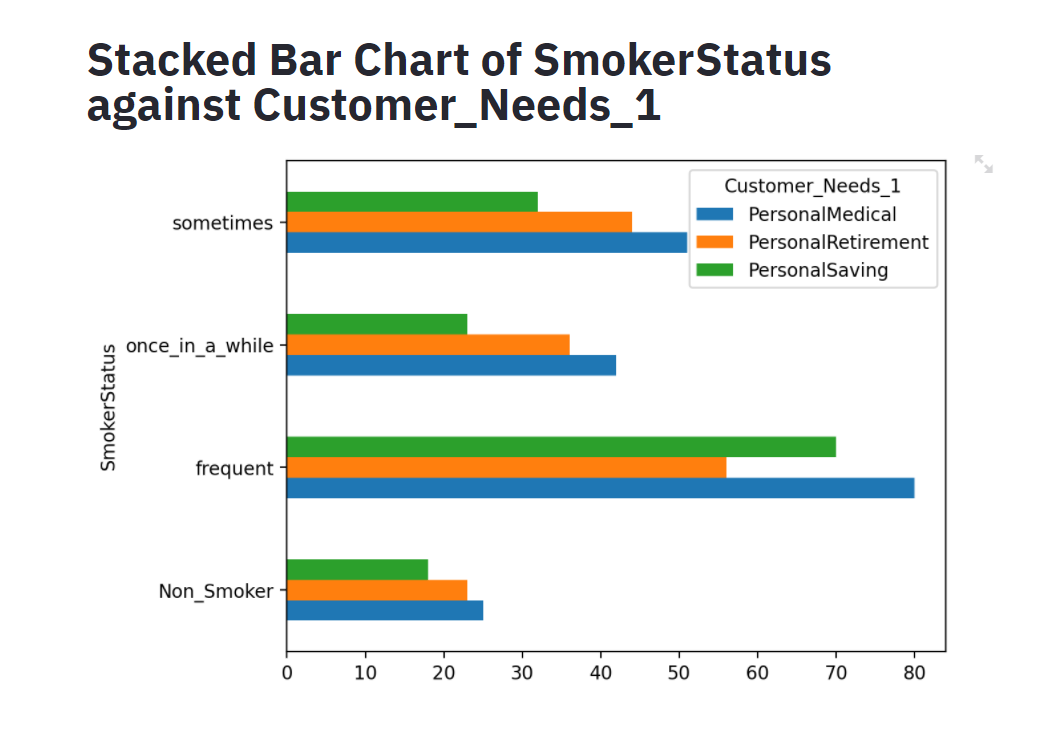
\includegraphics[width=1.00\textwidth]{diagram2.png}
     \caption{Smoker Status against Customer\_Needs\_1}
     \label{fig:diagram2.png}
 \end{figure}
\vspace{0.3cm}

 \begin{figure}[H] 
     \centering
     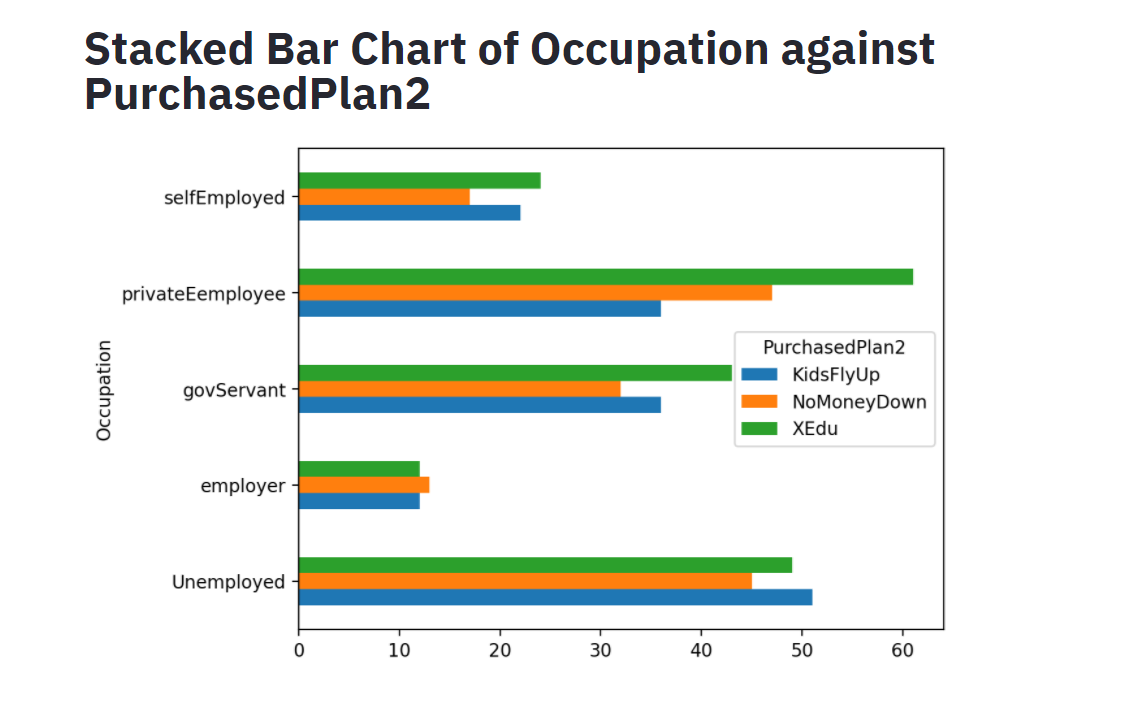
\includegraphics[width=1.00\textwidth]{diagram3.png}
     \caption{Occupation against PurchasedPlan2}
     \label{fig:diagram3.png}
 \end{figure}
\vspace{0.3cm}

 \begin{figure}[H] 
     \centering
     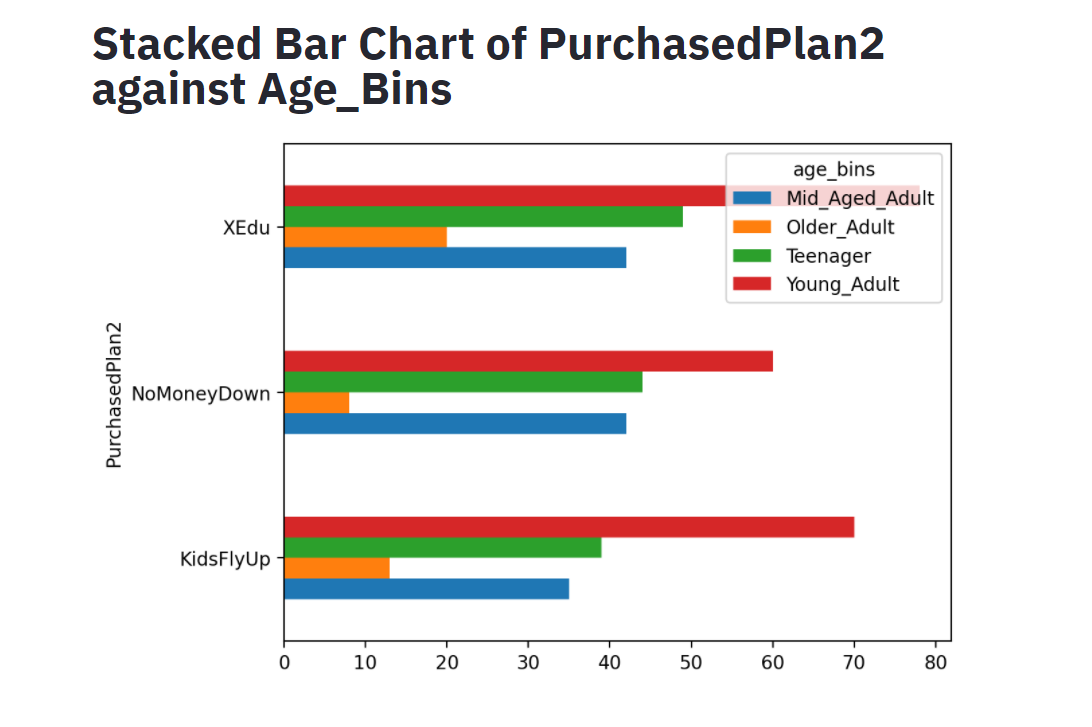
\includegraphics[width=1.00\textwidth]{diagram4.png}
     \caption{PurchasedPlan2 against Age\_Bins}
     \label{fig:diagram4.png}
 \end{figure}
\vspace{0.3cm}

 \begin{figure}[H] 
     \centering
     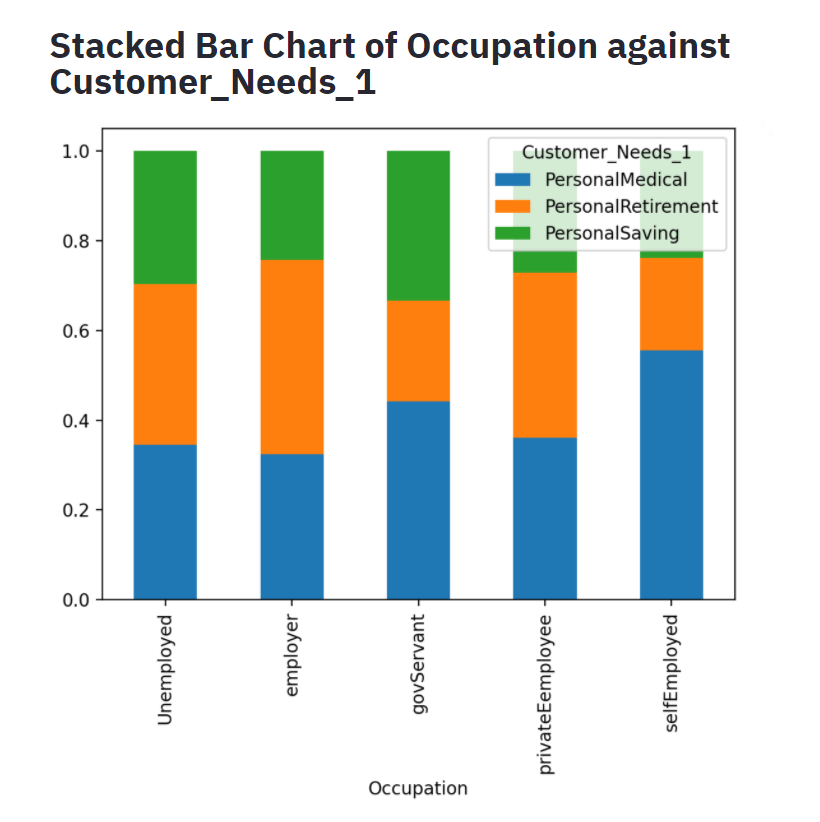
\includegraphics[width=1.00\textwidth]{diagram5.png}
     \caption{Occupation against Customer\_Needs\_1}
     \label{fig:diagram5.png}
 \end{figure}
\vspace{0.3cm}

 \begin{figure}[H] 
     \centering
     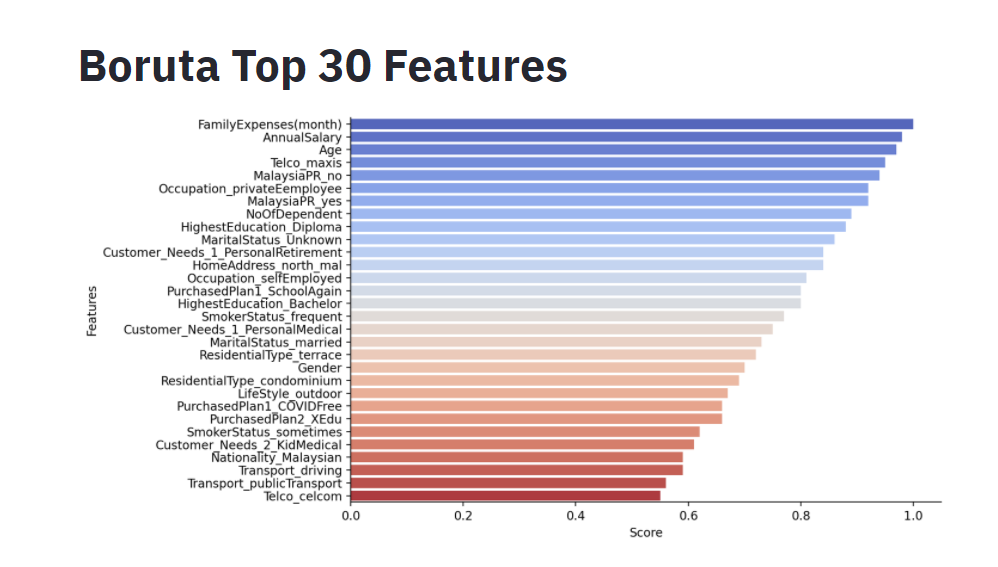
\includegraphics[width=1.25\textwidth]{diagram6.png}
     \caption{Boruta Top 30 Features}
    \label{fig:diagram6.png}
 \end{figure}
\vspace{0.3cm}

 \begin{figure}[H] 
     \centering
     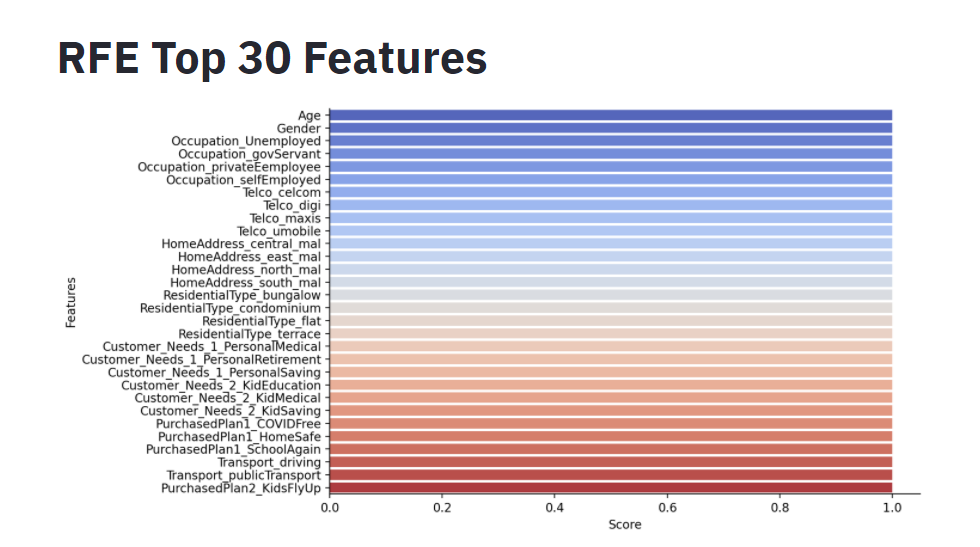
\includegraphics[width=1.25\textwidth]{diagram7.png}
     \caption{RFE Top 30 Features}
     \label{fig:diagram7.png}
 \end{figure}
 
  \begin{figure}[H] 
     \centering
     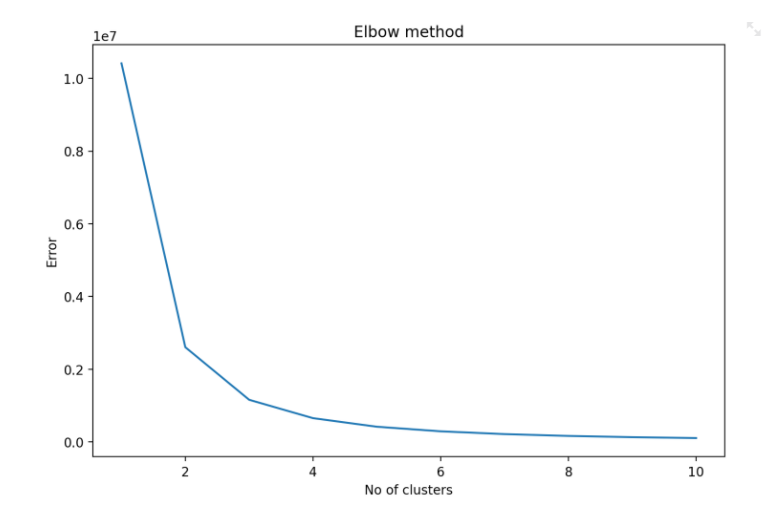
\includegraphics[width=0.95\textwidth]{diagram8.png}
     \caption{Elbow Method}
     \label{fig:diagram8.png}
 \end{figure}

\vspace{0.3cm}
\vspace{0.3cm}
\end{document}
 